\documentclass[bibtotoc,liststotoc,BCOR5mm,DIV12]{scrbook}

% use this declaration to set specific page margins
%\usepackage[a4paper , lmargin = {2.7cm} , rmargin = {2.9cm} , tmargin = {2.7cm} , bmargin = {4.6cm} ]{geometry}
\usepackage[a4paper]{geometry}

\usepackage[ngerman, english]{babel}
\usepackage{bibgerm}       		% german references
\usepackage{inputenc} % german characters
\usepackage{graphicx} 				% it's recommended to use PDF images but you can use JPG or PNG as well
\usepackage{url}           		% format URLs
\usepackage{hyperref} 				% create hyperlinks
\usepackage[toc]{glossaries}
\usepackage{listings, color}	% for source code
\usepackage{subfig}						% two figures next to each other (example: figure 3a), figure 3b)
\usepackage{scrpage2}					% header and footer line
\usepackage{array}
\newcolumntype{C}[1]{>{\centering\let\newline\\\arraybackslash\hspace{0pt}}m{#1}}
\usepackage{fancyref}

% header and footer line - no header & footer line on pages where a new chapter starts
\pagestyle{scrheadings}
\ohead{Techniques for Hierarchical Product Classification}
\ihead{Marilyn Nowacka Barros}
\ofoot[]{\thepage}
\ifoot{Master Thesis, TU Berlin, 2016}

% set path where images are stored
\graphicspath{{img/}}

%
% der Befehl \hypenation versteht keine Sonderzeichen, also weder �
% noch "a noch \"a. W�rter die derartige Zeichen enthalten m�ssen
% direkt im Text getrennt werden, z.B. W�r\-ter
%
\hyphenation{te-le-com-muni-cation 
te-le-com-muni-cation-specific 
Te-le-kom-mu-ni-ka-tions-API} 					% use this file to set explicit hyphenations (doesn't seem to work correctly)

\makeglossaries

\newglossaryentry{Linux}
{
  name=Linux,
  description={is a generic term referring to the family of Unix-like
               computer operating systems that use the Linux kernel},
  plural=Linuces
}


\begin{document}
% ---------------------------------------------------------------
\frontmatter
    \thispagestyle{empty}
\begin{center}

\vspace*{1.4cm}
{\LARGE \textbf{Technische Universit\"at Berlin}}

\vspace{0.5cm}

{\large Institute of Software Engineering and Theoretical Computer Science\\[1mm]}
{\large Database Systems and Information Management (DIMA)\\[5mm]}

Fakult\"at IV\\
Marchstr. 23,\\
10587 Berlin\\

\vspace*{1cm}


\includegraphics[width=4cm]{tu_logo.jpg}

\vspace*{1.0cm}

{\LARGE Master Thesis}\\

\vspace{1.0cm}
{\LARGE \textbf{Techniques for Hierarchical}}\\
\vspace*{0.3cm}
{\LARGE \textbf{Product Classification}}\\
\vspace*{1.0cm}
{\LARGE Marilyn Nowacka Barros}
\\
\vspace*{0.5cm}
Matriculation Number: 365912\\
\today\\ % 	date of submission
\vspace*{1.0cm}

Advisors\\
Juan Soto (DIMA, TU Berlin)\\
Jan Anderssen (idealo Internet GmbH)\\
\vspace*{0.5cm}
Reviewer\\
Prof. Dr.Volker Markl
\vspace{3cm}


\end{center}


   	\thispagestyle{empty}
    \cleardoublepage
    
   % \thispagestyle{empty}
\vspace*{3cm}


\begin{center}

\includegraphics[width=0.4\textwidth]{fokuspng.png}
\end{center}

\vspace*{0.2cm}

\begin{center}
FOKUS Institute\\
Kaiserin-Augusta-Allee 31\\
10589 Berlin\\
\end{center}
\vspace*{0.5cm}

\noindent This dissertation originated in cooperation with the Fraunhofer Institute for Open Communication Systems (FOKUS).

\vspace*{1cm}
\noindent 
First of all I would like to thank Prof. Dr. Thomas Magedanz at the Fraunhofer Institute FOKUS for giving me the opportunity to carry out state of the art research in this field. 
\\
\\
Special thanks to Mister X and Mister Y for their guidance. --- Some personel words... ---
\\
\\
Furthermore I would like to thank ...
   % \thispagestyle{empty}
   % \cleardoublepage
    
    \newpage

\thispagestyle{empty}

\begin{large}

\vspace*{6cm}

\noindent
Hereby I declare that I wrote this thesis myself with the help of no more than the mentioned literature and auxiliary means.
\vspace{2cm}

\noindent
Berlin, \today

\vspace{3cm}

\hspace*{7cm}%
\dotfill\\
\hspace*{8cm}%
\textit{(Signature M. Nowacka Barros)}

\end{large}
 
    \thispagestyle{empty}
    \cleardoublepage
    
    
    \thispagestyle{empty}
\vspace*{1.0cm}

\begin{center}
    \textbf{Abstract}
\end{center}

\vspace*{0.5cm}

\noindent
This template is intended to give an introduction of how to write diploma and master thesis at the chair 'Architektur der Vermittlungsknoten' of the Technische Universit�t Berlin. Please don't use the term 'Technical University' in your thesis because this is a proper name. 
\\
\\
On the one hand this PDF should give a guidance to people who will soon start to write their thesis. The overall structure is explained by examples. On the other hand this text is provided as a collection of LaTeX files that can be used as a template for a new thesis. Feel free to edit the design.
\\
\\
It is highly recommended to write your thesis with LaTeX. I prefer to use Miktex in combination with TeXnicCenter (both freeware) but you can use any other LaTeX software as well. For managing the references I use the open-source tool jabref. For diagrams and graphs I tend to use MS Visio with PDF plugin. Images look much better when saved as vector images. For logos and 'external' images use JPG or PNG. In your thesis you should try to explain as much as possible with the help of images.
\\
\\
The abstract is the most important part of your thesis. Take your time to write it as good as possible. Abstract should have no more than one page. It is normal to rewrite the abstract again and again, so  probaly you won't write the final abstract before the last week of due-date. Before submitting your thesis you should give at least the abstract, the introduction and the conclusion to a native english speaker. It is likely that almost no one will read your thesis as a whole but most people will read the abstract, the introduction and the conclusion.
\\
\\
Start with some introductionary lines, followed by some words why your topic is relevant and why your solution is needed concluding with 'what I have done'. Don't use too many buzzwords. The abstract may also be read by people who are not familiar with your topic.
    \thispagestyle{empty}
    \cleardoublepage
    
    \thispagestyle{empty}
\vspace*{0.2cm}

\begin{center}
    \textbf{Zusammenfassung}
\end{center}

\vspace*{0.2cm}

\noindent 
Da die meisten Leuten an der TU deutsch als Muttersprache haben, empfiehlt es sich, das Abstract zus�tzlich auch in deutsch zu schreiben. Man kann es auch nur auf deutsch schreiben und anschlie�end einem Englisch-Muttersprachler zur �bersetzung geben.
    \thispagestyle{empty}
    
    
    \tableofcontents
    \thispagestyle{empty}
    
    \listoffigures
    \thispagestyle{empty}
    
    \listoftables
    \thispagestyle{empty}
    
% --------------------------------------------------------------

\mainmatter % comment single chapters for faster compilation

    \chapter{Introduction\label{cha:intro}}
%4-8 pages
\gls{Linux}

Nowadays, consumers are increasingly opting to shop online. However, with so many retailers offering products online, arguably, consumers need better solutions to help them identify the specific product they would like to purchase at the lowest possible price. Commonly, retailers categorize consumer products, according to varying schemes (e.g., based on a company-specific taxonomy) and performing classification using manual or automated means. Unfortunately, these methods are not entirely accurate. Therefore, in this master's thesis, we aim to use machine learning techniques for multiclassification of online products and map them to a taxonomy of categories. As a by-product, this would likely also help to improve the detection of product duplicates and discover complementary product recommendations [1]. 

Despite the wide variety of existing eCommerce platforms, they all share one thing in common, i.e., the need to automatically classify their product offerings into a hierarchical taxonomy. Some research has already been done in this area by Yahoo! ([1]), eBay ([2, 3, 4]), and also outside of e-Commerce (e.g., performing hierarchical classification on web content [5]). As proposed in [2,3,5], when a hierarchical taxonomy is employed as target for classification, we could vary the set of product features or the particular multiclassification algorithm, depending on the level of the tree we are classifying into. However, to the best of my knowledge, combining the previous strategy with typical machine learning classification algorithms (e.g., SVM, kNN) has not been tried using large-scale data processing engines, such as Apache Flink or Apache Spark (e.g., to shorten runtimes and reduce training times). Indeed, there is a lot of room for improvement (e.g., increasing classification accuracy, reducing analysis times, and facilitating conducting benchmarks).

One of Germany's largest price comparison platform (idealo ([6]) offers consumers varying navigation options. Users are able to browse almost 2 million products that are labeled using more than 2000 different categories. These categories are organized into a hierarchical taxonomy, where products can be compared at a glance. For example, a Coleman Tent is classified as Leisure \& Outdoors > Camping > Tent, i.e., a Coleman Tent is classified as a Tent, which is a category that belongs to Camping, and at the same time is in the Leisure \& Outdoors’ category. Designing and implementing a system that can automatically organize products into a broad set of categories accurately is a non-trivial task.
Due to the large amounts of data handled by e-Commerce platforms every day, we need a multiclassification algorithm that can run on a large-scale data analytics system, like Spark or Flink. This should enhance runtime efficiency and offer a scalable solution. 



\section{Motivation\label{sec:moti}}

Start describing the situation as it is today or as it has been during the last years. 'Over the last few years there has been a tendency... In recent years...'. The introduction should make people aware of the problem that you are trying to solve with your concept, respectively implementation. Don't start with 'In my thesis I will implement X'.

\section{Objective\label{sec:objective}}

What kind of problem do you adress? Which issues do you try to solve? What solution do you propose? What is your goal?
'This thesis describes an approach to combining X and Y... The aim of this work is to...'

\section{Scope\label{sec:scope}}

Here you should describe what you will do and also what you will not do. Explain a little more specific than in the objective section. 'I will implement X on the platforms Y and Z based on technology A and B.'

Conclude this subsection with an image describing 'the big picture'. How does your solution fit into a larger environment? You may also add another image with the overall structure of your component.

'Figure \ref{fig:intro} shows Component X as part of ...' 
\\
\begin{figure}[htb]
  \centering
  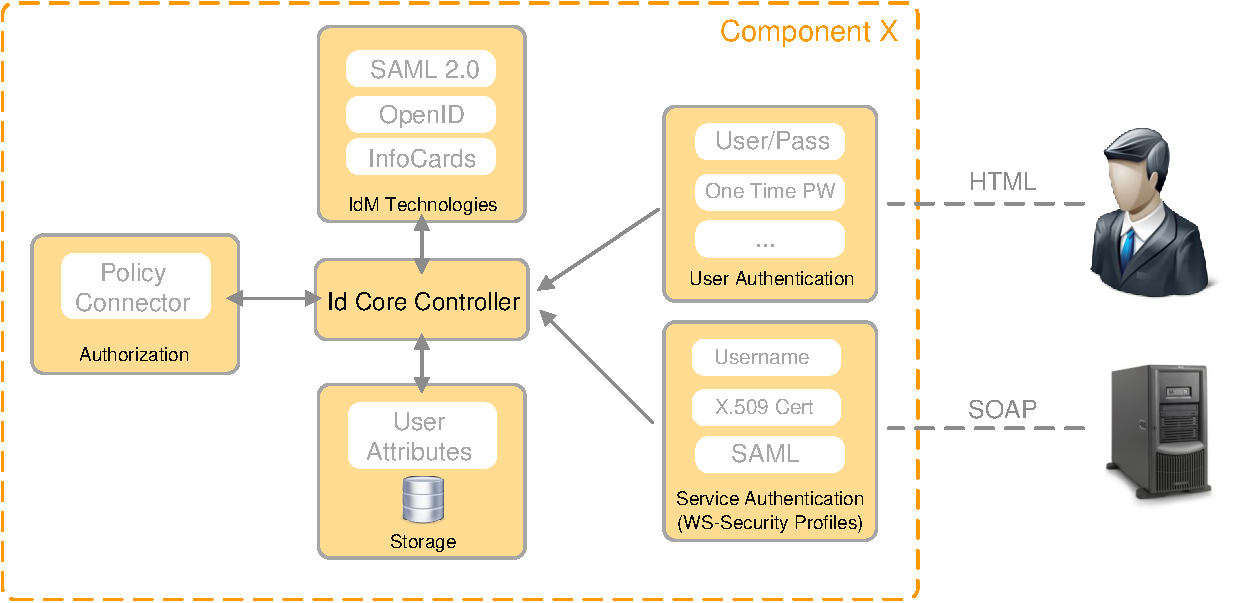
\includegraphics[width=9cm]{intro_example.pdf}\\
  \caption{Component X}\label{fig:intro}
\end{figure}

\begin{figure}[htb]
  \centering
  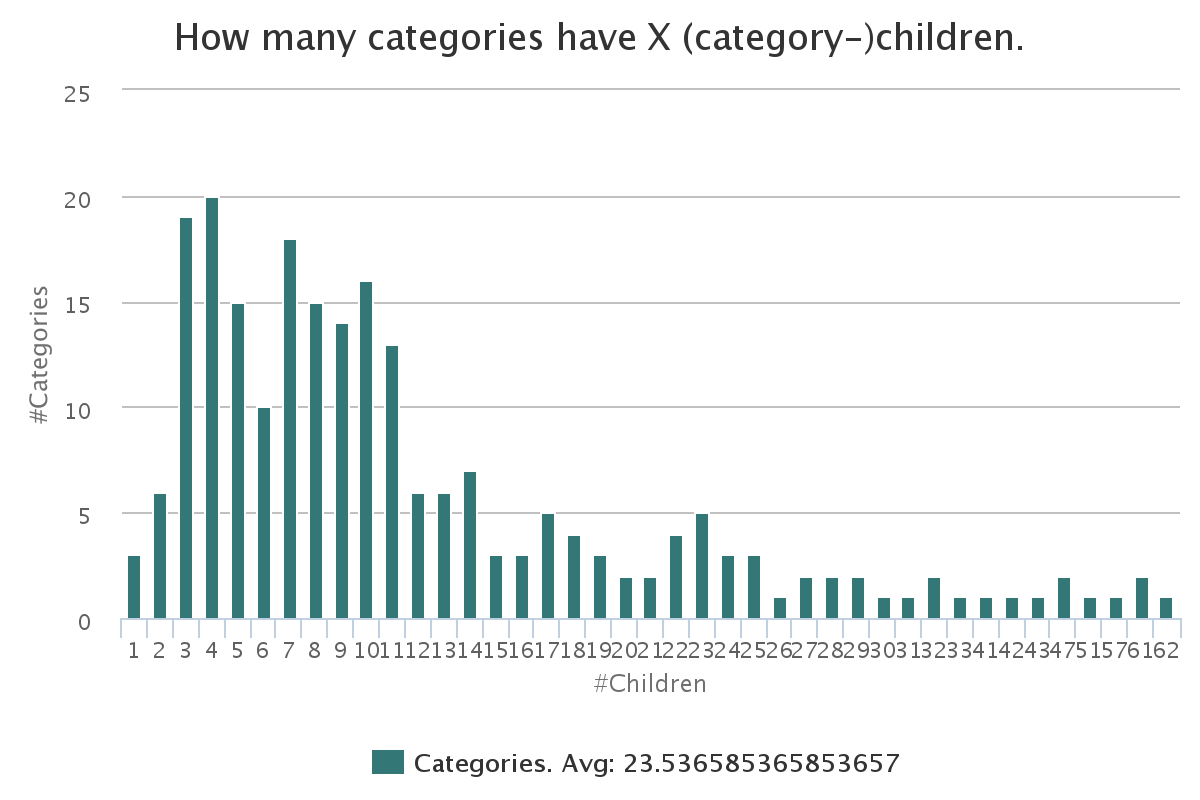
\includegraphics[width=15cm]{/plots/statistics/outdegreeCats.png}\\
  \caption{Outdegree}\label{fig:outdegree}
\end{figure}

\section{Structure\label{sec:outline}}

This Thesis is presented in X chapters:
\\
\\
\noindent This example thesis is separated into 7 chapters.
\\
\\
\textbf{Chapter \ref{cha:tf}} is usually termed 'Related Work', 'State of the Art' or 'Fundamentals'. Here you will describe relevant technologies and standards related to your topic. What did other scientists propose regarding your topic? This chapter makes about 20-30 percent of the complete thesis.
\\
\\
\textbf{Chapter \ref{cha:idealo}} analyzes the requirements for your component. This chapter will have 5-10 pages.
\\
\\
\textbf{Chapter \ref{cha:chapter4}} is usually termed 'Concept', 'Design' or 'Model'. Here you describe your approach, give a high-level description to the architectural structure and to the single components that your solution consists of. Use structured images and UML diagrams for explanation. This chapter will have a volume of 20-30 percent of your thesis.
\\
\\
\textbf{Chapter \ref{cha:chapter5}} describes the implementation part of your work. Don't explain every code detail but emphasize important aspects of your implementation. This chapter will have a volume of 15-20 percent of your thesis.
\\
\\
\textbf{Chapter \ref{cha:chapter6}} is usually termed 'Evaluation' or 'Validation'. How did you test it? In which environment? How does it scale? Measurements, tests, screenshots. This chapter will have a volume of 10-15 percent of your thesis.
\\
\\
\textbf{Chapter \ref{cha:chapter7}} summarizes the thesis, describes the problems that occurred and gives an outlook about future work. Should have about 4-6 pages.
    \chapter{Fundamentals and Related Work\label{cha:tf}}

Multiclassification has been topic that has been explored frequently in a diverse number of fields. 
...
 Next we present some of the related work done in this are of knowledge:
\subsection{Text Categorization (Natural Language Processing)}
If movies were Computer Science, and actors and their lives were the different topics and fields of study in Computer Science, Machine Learning would be something like the Kardashians. Everyone has heard of it, everyday there are news about it and not everyone really knows what's really going on. 
Multiclassification and Multilabels....
\subsection{Scalable Data Algorithms}
With the nowadays always increasing amount of data, the need of mechanisms to proccess and deal with the data we are producing, and need to consume is needed.
book, scale, distribution, spark
\subsection{Taxonomy in the web}
flat vs hierarchical

\section{Technologies \label{sec:tech}}

This section describes relevant technologies, starting with X followed by Y, concluding with Z.

\subsection{Technology A\label{sec:aaa}}

It's always a good idea to explain a technology or a system with a citation of a prominent source, such as a widely accepted technical book or a famous person or organization. 

Exmple: Tim-Berners-Lee describes the ''WorldWideWeb'' as follows:
\\
\textit{''The WorldWideWeb (W3) is a wide-area hypermedia information retrieval initiative aiming to give universal access to a large universe of documents.''} \cite{timwww}
\\
\\
You can also cite different claims about the same term.
\\
According to Bill Gates \textit{''Windows 7 is the best operating system that has ever been released''} \cite{billgates} (no real quote)
In opposite Steve Jobs claims Leopard to be \textit{''the one and only operating system''} \cite{stevejobs}

If the topic you are talking about can be grouped into different categories you can start with a classification.
Example: According to Tim Berners-Lee XYZ can be classified into three different groups, depending on foobar \cite{timwww}:
	\begin{itemize}
		\item Mobile X
				\vspace{-0.1in} 
		\item Fixed X
				\vspace{-0.1in} 
		\item Combined X
 	\end{itemize}

\subsection{Technology B\label{sec:bbb}}

For internal references use the 'ref' tag of LaTeX. Technology B is similar to Technology A as described in section \ref{sec:aaa}.

\newpage

\subsection{Comparison of Technologies\label{sec:comp}}

\begin{table}[htb]
\centering
\begin{tabular}[t]{|l|l|l|l|}
\hline
Name & Vendor & Release Year & Platform \\
\hline
\hline
A & Microsoft & 2000 & Windows \\
\hline
B & Yahoo! & 2003 & Windows, Mac OS \\
\hline
C & Apple & 2005 & Mac OS \\
\hline
D & Google & 2005 & Windows, Linux, Mac OS \\
\hline
\end{tabular}
\caption{Comparison of technologies}
\label{tab:enghistory}
\end{table}

\section{Standardization \label{sec:standard}}

This sections outlines standardization approaches regarding X.

\subsection{Internet Engineering Task Force\label{sec:itu}}

The IETF defines SIP as '...' \cite{rfcsip}

\subsection{International Telecommunication Union\label{sec:itu}}

Lorem Ipsum...

\subsection{3GPP\label{sec:3gpp}}

Lorem Ipsum...

\subsection{Open Mobile Alliance\label{sec:oma}}

Lorem Ipsum...

\section{Concurrent Approaches \label{sec:summ}}

There are lots of people who tried to implement Component X. The most relevant are ...
    \chapter{Requirements\label{cha:idealo}}
Explore new techniques or alternatives for classification.

\section{Difficulty of The Problem\label{sec:reqoverview}}
IN GENERAL. Why is in general difficult to classify stuff...

VCR/Subjectivity: real categories are set by humans. Too much subjectivity. 


\section{Technical Requirements\label{sec:techreq}}
Taxonomy is already made. No matter if it makes sense. 

\subsection{Sub-component A\label{sec:reqsuba}}


\subsection{Sub-component B\label{sec:reqsubb}}

Lorem Ipsum...

\section{(Soft?)Social Requirements\label{sec:socreq}}

Component X must compete with Y. Hence, it is required to provide an excellent usability. This includes ... scalability, consistency, etc....
    \chapter{Analysis of the Data\label{cha:chapter4}}
%This chapter introduces the architectural design of Component X. The component consists of subcomponent A, B and C.

%In the end of this chapter you should write a specification for your solution, including interfaces, protocols and parameters.
Idealo has organised its products into a tree structure of categories. Each product is classified into a category. That is, having a set of target categories $C = {c_1, c_2, ..., c_t}$ and a set of products $P = {p_1, p_2, ..., p_n}$:

\begin{center}
    $(\forall p_i \in P, \exists c_j \in C : l(p_i) = c_j $)  \\
\end{center}

Where $l$ is function that maps a product to a category, such that:\\

\begin{center}
    $l: P \rightarrow C$. \label{eq:classifierFunction}\\
\end{center}

Categories are arranged in a human-elaborated tree structure, where categories in the upper levels of the tree are related to more general definitions (e.g. Telecommunications, Computer\&Hardware, Fashion\&Accessories...), and leaves or categories in deeper levels represents more specific categories (e.g: Red Wines, Bank Benches, Footballs...).For example, \textit{Pictonary} is a famous and nice board game, this is how it looks part of its page at idealo's website (see figure \ref{fig:pictionary})

\begin{figure}[!htbp]
  \centering
  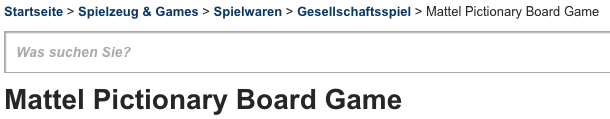
\includegraphics[width=10cm]{pictionary.png}\\
  \caption{Path of categories for a product}
  \label{fig:pictionary}
\end{figure}

\textit{Pictonary} is classified as a \textit{Gesellschaftsspiel} (board game). It's important to notice, that we can see already in the interface of the website that this category has \textit{Spielwaren} (toys) as its parent in the category tree, and the latter is a child of the \textit{Spielzeug\&Games} (toys and games) category, which is a first level category (\textit{Startseite} is the root).

Notice that products can belong to any category in the tree (i.e. classification is not exclusive into leaf categories, but also node categories). Figure \ref{fig:idealoTree} shows a general overview of the structure of the category tree.

\begin{figure}[!htbp]
  \centering
  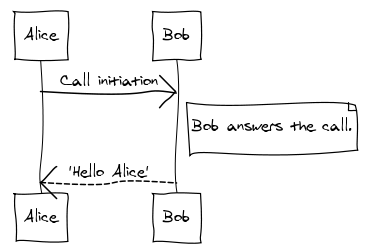
\includegraphics[width=9cm]{uml_seq_example.png}\\
  \caption{Category Tree}
  \label{fig:idealoTree}
\end{figure}


\section{Where does the Classifier fit?\label{sec:classifier}}
%Explain where is situated the classifier in the Idealo's structure or the path of an offer.
The route a product follows since it is retrieved from an online-shop till it is showed to the final user in the website is a long path. After a product is retrieved, it's determined whether it's a new product or something that has been seen before by trusted classification processes. Also, a set of rules are employed to reduce the amount of products that need to be classified (knowledge engineering). Then, after some products are already out, X\% makes it to the classifier that uses machine learning techniques. 
For the classifier's decision to be taken into account, it needs to have 80\% of confidence in the answer it's giving.
Products that aren't classified by any of this stages are manually classified by domain experts (i.e. items that had less than 80\% of confidence in the classifier).

The classifier is a supervised learning algorithm that assigns a unique label (category) to every given datapoint (product) (See equation ~\ref{eq:classifierFunction}). From now on, we will assume we are only inside the classifier context (i.e. products and categories are those that the classifier knows).

\section{The Categories \label{sec:conceptsubb}}

%Structure of the categories, the taxonomy, distributions, etc.
All categories are structured into a category tree that was built by domain experts. Nodes and leaves from the tree are categories that may be target-categories. 
When a product is assigned to one target-category, it means that this product also (implicitly) belongs to all the categories that conform the path from this (target-)category up to the root of the tree. For example, given the subtree in figure \ref{fig:subtree}, a product that was assigned to be in the \textit{Art} target-category, would be implicitly  belong to \textit{Culture} and \textit{Encyclopedia} (root) too.

\begin{figure}[!htbp]
  \centering
  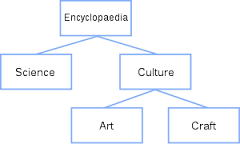
\includegraphics[width=9cm]{treeEx.png}\\
  \caption{SubTree}
  \label{fig:subtree}
\end{figure}

As said before, products aren't exclusively classified into leaf categories (i.e. node-categories are sometimes subject of classification too). Let's say we have an Encyclopedia for Cultural Expressions. This product fits exactly in the \textit{Culture} category, therefore this product should be classified as \textit{Culture}. Nevertheless this is implicitly also classified as \textit{Encyclopedia}, as it's parent of the target-category \textit{Culture}. 

Now that we have understood intuitively this concepts, let's built a mathematical definition out of it. Let $C$ be a set containing all categories, $C = {c_1, c_2, ..., c_t}$ and $P$ the set of products $P = {p_1, p_2, ..., p_n}$. Let $R = {r_1, r_2..., r_t}$ be a set that contains the root paths of all categories in $C$, that is $r_i \subseteq C$ is a set that contains the path from the root of the tree to the node/leaf $c_i$. Then, when a product $p_j$ is classified as $c_i$ ($l(p_j) = c_i$), implicitly, $p_j$ also belongs to all categories in $r_i$.

Then, the classifier ($l: P \rightarrow C$) should select the target-category that first suites better a product, and second its located in the highest level of the tree of categories (i.e. the most suitable deepest category in the tree).

\subsection{The Taxonomy}
%explain the taxonomy, the fact that a category can be a node AND a category subject of classification (not only leaves).
The Categories' taxonomy is a very wide tree with 6 levels. It presents a very uneven distribution of the categories among its branches (see figure \ref{fig:distCats}). As seen in table \ref{tab:categoryDist}, the first level of the tree contains 13 categories. All of this 13 categories (there are 0 leaves at this level), have in average 11 children. The first-level category with less children contains 8, and the one with most have 16. X out of 13 are target categories in the first category (i.e. products are classified into those).
In the last level of the tree, there's only 4 leaf-categories.

\begin{figure}[!htbp]
  \centering
  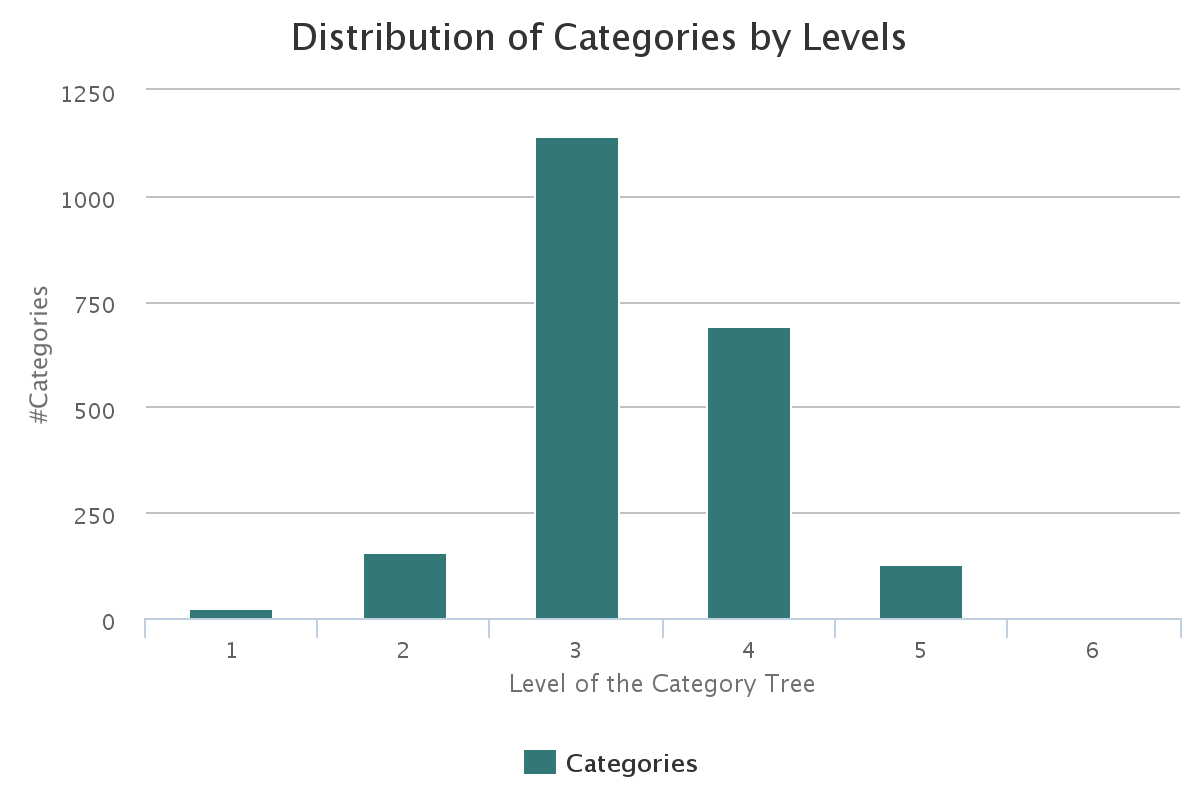
\includegraphics[width=14cm]{DistCatsLevels.png}\\
  \caption{Distribution of Categories across levels of the category tree}
  \label{fig:distCats}
\end{figure}

\begin{table}[!htbp]
    \centering
    \begin{tabular}{|c|c| C{1.5cm} | C{1.5cm} | C{1.5cm}| C{1.5cm}|C{1.5cm}|}
       \hline
       Level &  X-Level & \multicolumn{5}{c|}{Category Node Withing Level-X Nodes} \\
       \cline{3-7}
         & Categories & Avg & Min & Max & Leaves & Target  \\
       \hline
        1 & 13 & 11 & 8 & 16 & 0 & \\
        2 & 152 & 11 & 47 &1 & 52 & \\
        3 & 1138 & 8 & 46 & 1 & 1056&  \\
        4 & 686 & 6 & 12 & 2 & 663& \\
        5 & 128 & 4 & 4 & 4 & 127& \\
        6 & 4 & 0 & 0 & 0 & 4 & 4 \\
        \hline
        
    \end{tabular}
    \caption{Distribution of Categories in the Category Tree}
    \label{tab:categoryDist}
\end{table}


\section{The Products\label{sec:conceptsubb}}

%Structure of Angebote, relation with categories
Products have several features that can be used for the classification task. The main problem about this, is that it consists of a very heterogenuos representation: not always all features exist in all products.
From all existent features, this are the one that were chosen for this project
\begin{itemize}
    \item Title: this is one of the features that products lack the less. It's the title of a product that is retrieved from the retailers. It's a text field, that on average has 11 words.
    \item Description: this text field describe or explain what the product is.
    \item Brand: the brand of the product
    \item Attributes: a list of attributes that a product has (such as size, in the case of shoes, RAM in the case of computers, etc.). There are up to 8005 different alternatives for attributes.
    \item productSearchText:
    \item shopKategorie:
\end{itemize}

From the uneven distribution of categories across levels in the tree, it's already expected that the products are also unevenly distributed across levels in the tree. This is confirmed in figure \ref{fig:productsDist}
\begin{figure}[!htbp]
  \centering
  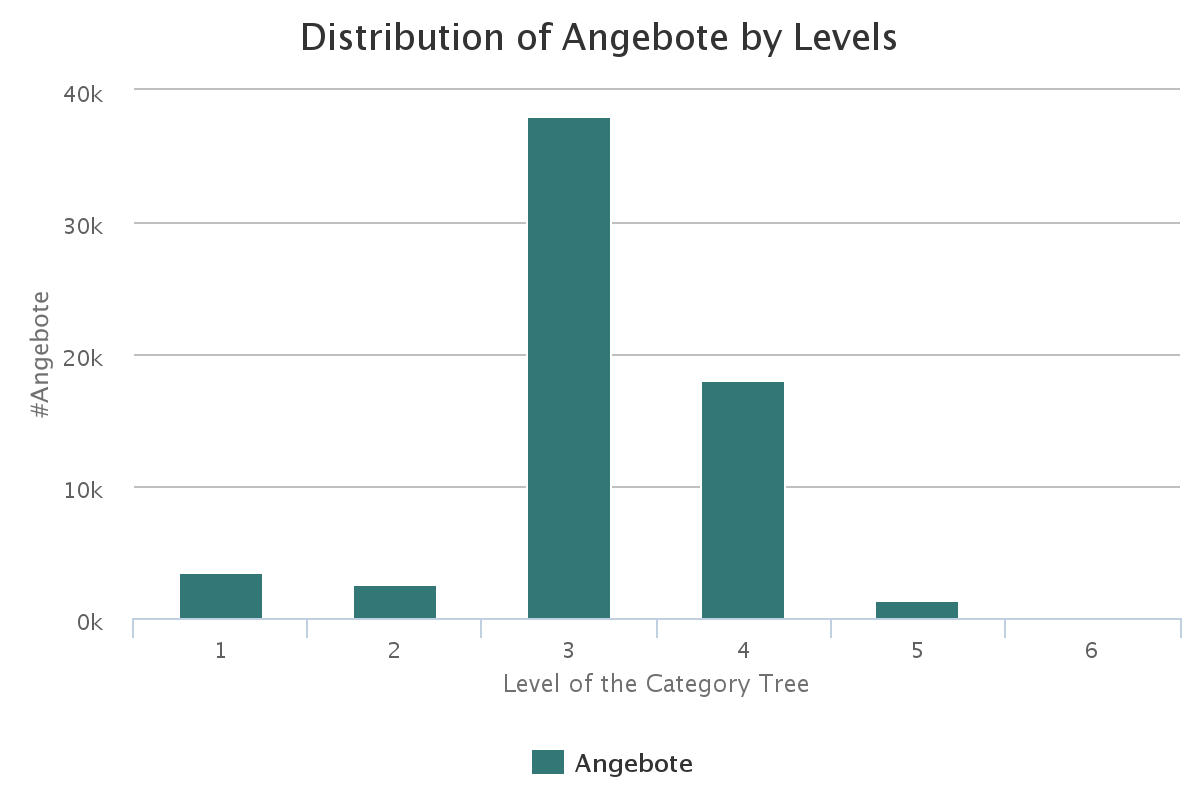
\includegraphics[width=14cm]{DistAngeLevels.png}\\
  \caption{Distribution of Products across levels of the category tree}
  \label{fig:productsDist}
\end{figure}

This uneven distribution is not just across levels in the tree, also includes the outdegree of categories (see figure \ref{fig:distProdCats})

\begin{figure}[!htbp]
  \centering
  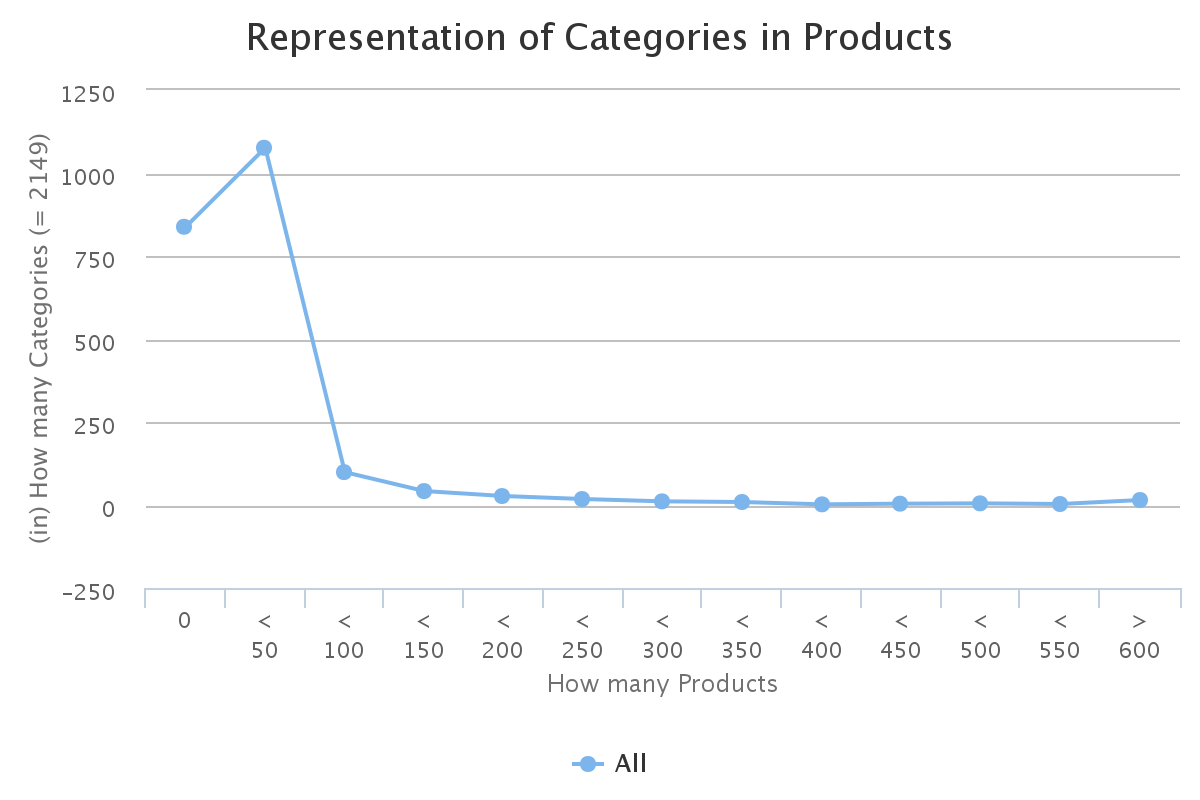
\includegraphics[width=14cm]{DistProductsOverCats2.png}\\
  \caption{Distribution of Products over Categories}
  \label{fig:distProdCats}
\end{figure}

\section{Problems with the Data\label{sec:conceptlayerx}}
Natural language problems: misspelling, german umlaut. 
Not balanced Data: Distribution... (pic)
Irregularities in Data: other alphabet (japanesse, corean...), IDs,

Uneven distribution, LinkedTarget, empty features, ghost categories, lack of quality for some classified products (misclassified in training data)...EXAMPLES!. 

Classification of misspelled stuff

\section{The Classification Task}
General explanation based on the showed plots, how will be classified the data (e.g. coarse-grained approach), play with features at each level.

\section{Place of Work\label{sec:conceptinter}}

Cluster, PC, etc (memory, OS, processors, etc)

\section{Spark with Scala\label{sec:intspec}}

Lorem Ipsum...


    \chapter{Implementation\label{cha:chapter5}}



\section{Environment\label{sec:env}}
The following software, respectively operating systems, were used for the implementation:

\begin{itemize}
		\item and Ubuntu 6
		\vspace{-0.1in} 
		\item Scala X
		\vspace{-0.1in} 
		\item IntelliJ X
		\vspace{-0.1in} 
		\item Spark X
		\vspace{-0.1in} 
		\item jUnit X
		\vspace{-0.1in} 
		\item ....check POM for more versions
\end{itemize}

\section{General Project Structure\label{sec:projectstructure}}

The Implementation has 4 marked phases that can be seen easily in the pipeline that a test needs to follow.. PICTURE

\section{Preprocessing}
linkedTarget, create virtual categories for the one that contains products: decision of which ID to put them. 
Better structures, titles with AT and DE sometimes...

\section{Feature Modeling}
Which features, what was done
tokens (by empty spaces)
gr\"osse gr\"oße example

attributeTextSearch

 8005 lenght. 
 1. Binary dense vector
 2. Sparse vector of hashes
 3. Concatenate names.

\section{Word2Vector}
Explain the model.

\section{Classification: kNN}
In general KNN

\subsection{Implementation of KNN\label{sec:gui}}

Structure of the algorithm. Screenshot of spark's visualization tool. 
How many shuffles. Etc.

Selection of k. Dinamically (as proposed somewhere), doesnt make any change, because top2 is almost always below suggested threshold and for finding a threshold by our own, would be so time consuming (?)

\lstset{caption=JSON String Code Snippet,label=jsonstring,showstringspaces=false}
\begin{lstlisting}
{
	id: 1,
	method: "myInstance.getGroup",
	params: ["Teammates", 2, true]
}

{
	id: 2,
	result: [
		  "groupDesc":"These are my teammates",
		  {
			"javaClass":"src.package.MemberClass",
			"memberName": "Bob",      
		  }
		]
}\end{lstlisting}

\section{Classification: SVM}
Explain SVM

\subsection{SVM in Spark}
Explain their implementation

\section{One Against All}
Explain what is that, why is it prefered

\subsection{Implementation of OAA}
Explain my implementation

\section{Cross Validation}
Explain my/their implementation

\section{Evaluation}
Evaluation methods explanation

\section{Documentation\label{sec:docu}}

Everything was documented with scaladocs.



    \chapter{Evaluation\label{cha:chapter6}}

In this chapter the implementation of Component X is evaluated. An example instance was created for every service. The following chapter validates the component implemented in the previous chapter against the requirements.
\\
\\
Put some screenshots in this section! Map the requirements with your proposed solution. Compare it with related work. Why is your solution better than a concurrent approach from another organization?

\section{Test Environment\label{sec:testenvir}}

Fraunhofer Institute FOKUS' Open IMS Playground was used as a test environment for the telecommunication services. The IMS Playground ...

\section{Scalability\label{sec:scal}}

Lorem Ipsum

\section{Usability\label{sec:usab}}

Lorem Ipsum

\section{Performance Measurements\label{sec:performance}}

Lorem Ipsum
    \chapter{Conclusion\label{cha:chapter7}}
The final chapter summarizes the thesis. The first subsection outlines the main ideas behind Component X and recapitulates the work steps. Issues that remained unsolved are then described. Finally the potential of the proposed solution and future work is surveyed in an outlook.

\section{Summary\label{sec:summary}}

Explain what you did during the last 6 month on 1 or 2 pages!
\\
\\
\noindent The work done can be summarized into the following work steps

\begin{itemize}
		\item Analysis of available technologies
		\vspace{-0.11in} 
		\item Selection of 3 relevant services for implementation
		\vspace{-0.11in} 
		\item Design and implementation of X on Windows
		\vspace{-0.11in} 
		\item Design and implementation of X on mobile devices
		\vspace{-0.11in} 
		\item Documentation based on X
		\vspace{-0.11in} 
		\item Evaluation of the proposed solution
\end{itemize}

\section{Dissemination\label{sec:dissemination}}

Who uses your component or who will use it? Industry projects, EU projects, open source...? Is it integrated into a larger environment? Did you publish any papers?

\section{Problems Encountered\label{sec:problems}}

Summarize the main problems. How did you solve them? Why didn't you solve them?

\section{Outlook\label{sec:outlook}}

Future work will enhance Component X with new services and features that can be used ...


% ---------------------------------------------------------------
\backmatter % no page numbering from here
    %\addchap{Dictionary}
\gls{Linux}
\newglossaryentry{Linux}
{
  name=Linux,
  description={is a generic term referring to the family of Unix-like
               computer operating systems that use the Linux kernel},
  plural=Linuces
}


\glsaddall

    \printglossaries
    \addchap{List of Acronyms}

\begin{tabbing}
spacespacespace \= space \kill
3GPP	 \> 	3rd Generation Partnership Project	 \\
AJAX	\>	Asynchronous JavaScript and XML \\
API	 \> 	Application Programming Interface	 \\
AS	\>	Application Server \\
CSCF	 \> 	Call Session Control Function	 \\
CSS	\>	Cascading Stylesheets \\
DHTML	\>	Dynamic HTML \\
DOM	\>	Document Object Model \\
FOKUS	\>	Fraunhofer Institut fuer offene Kommunikationssysteme \\
GUI	\>	Graphical User Interface \\
GPS	\>	Global Positioning System \\
GSM	\>	Global System for Mobile Communication\\
HTML	\>	Hypertext Markup Language \\
HSS	 \> 	Home Subscriber Server	 \\
HTTP	 \> 	Hypertext Transfer Protocol	 \\
I-CSCF	 \> 	Interrogating-Call Session Control Function	 \\
IETF	\>	Internet Engineering Task Force \\
IM	\>	Instant Messaging \\
IMS	 \> 	IP Multimedia Subsystem	 \\
IP	 \> 	Internet Protocol	 \\
J2ME	\>	Java Micro Edition \\
JDK	\>	Java Developer Kit \\
JRE	\>	Java Runtime Environment \\
JSON	\>	JavaScript Object Notation \\
JSR	\>	Java Specification Request \\
JVM	 \> 	Java Virtual Machine	 \\
NGN	 \> 	Next Generation Network	 \\
OMA	 \> 	Open Mobile Alliance	 \\
P-CSCF	 \> 	Proxy-Call Session Control Function	 \\
PDA	\>	Personal Digital Assistant \\
PEEM	 \> 	Policy Evaluation, Enforcement and Management	 \\
QoS	 \> 	Quality of Service	 \\
S-CSCF	 \> 	Serving-Call Session Control Function	 \\
SDK	\>	Software Developer Kit \\
SDP	\>	Session Description Protocol \\
SIP	 \> 	Session Initiation Protocol	 \\
SMS	\>	Short Message Service \\
SMSC	\> Short Message Service Center \\
SOAP	 \> 	Simple Object Access Protocol	 \\
SWF	\>	Shockwave Flash \\
SWT	\>	Standard Widget Toolkit \\
TCP	 \> 	Transmission Control Protocol	 \\
Telco API	\>	Telecommunication API \\
TLS	\>	Transport Layer Security \\
UMTS	 \> 	Universal Mobile Telecommunication System	 \\
URI	 \> 	Uniform Resource Identifier	 \\
VoIP	 \> 	Voice over Internet Protocol	 \\
W3C	 \> 	World Wide Web Consortium	 \\
WSDL	\>	Web Service Description Language \\
XCAP	 \> 	XML Configuration Access Protocol	 \\
XDMS	 \> 	XML Document Management Server	 \\
XML	 \> 	Extensible Markup Language	 \\
\end{tabbing}
\endinput

    \chapter{Dictionary\label{cha:dict}}

\begin{itemize}
    \item Product: any good whose price is compared at the idealo's website (e.g. White Album from The Beatles).
    \item Category: class. We want to classify products into categories (e.g. Audio-Cds). The names are originally in German, therefore in this work it's translated into English.
    \item Category Tree: structure where categories are situated. Each node and leaf represents each category. A category is a child of other, when semantically one contains the other one (e.g. the category node "Schue" (shoes) is a child of the category node "Mode und Accessoires" (Fashion and Accessories).
    \item Super Category: category belonging to the first level of categories, in the category tree.
    \item Node Category: category that have at least one category child
    \item Leaf Category: category that doesn't have any child.
    \item Target Category: category that represent any product (i.e. there is at least one product, whose assigned category is the target category). Naturally, there are categories that aren't assigned to any product (always node categories).
    \item X-Level Category: category belonging to the level X of the category tree. Super Categories are First-Level categories. The deepest level is level 6. The root is level 0.
    \item Predicted Category: predicted class.
    \item Real Category: real class of a product
    \item Predicted Super Category: predicted first layer class.
\end{itemize}

TODO: Symbols dictionary


		
		% if you want to provide a glossary with explanations of important terms put it in here

    \bibliographystyle{geralpha}
    \bibliography{bib/references}
    
    \addchap{Annex}

\begin{appendix}

\lstset{language=,caption=Sourcecode Listing,captionpos=b,
label=yahoowidgetkon,showstringspaces=false,
basicstyle={\fontfamily{pcr}\selectfont\footnotesize}}
\begin{lstlisting}
<?xml version="1.0" encoding="UTF-8"?>
<widget>
	 <debug>off</debug>
	 <window name="myWindow" title="Hello Widget" visible="true">
		 <height>120</height>
		 <width>320</width>
		 <image src="Resources/orangebg.png">
			<name>orangebg</name>
			<hOffset>0</hOffset>
			<vOffset>0</vOffset>
		</image>
		 <text>
			 <name>myText</name>
			 <data>Hello Widget</data>
			 <color>#000000</color>
			 <size>20</size>
			 <vOffset>50</vOffset>
			 <hOffset>120</hOffset>
		 </text>
	</window>
</widget>
\end{lstlisting}

\newpage


\lstset{caption=SIP request and response packet\cite{SIPBook},
captionpos=b,label=sippacket,showstringspaces=false,
basicstyle={\fontfamily{pcr}\selectfont\footnotesize}}
\begin{lstlisting}
INVITE sip:bob@network.org SIP/2.0
Via: SIP/2.0/UDP 100.101.102.103:5060;branch=z9hG4bKmp17a
Max-Forwards: 70
To: Bob <sip:bob@network.org>
From: Alice <sip:alice@ims-network.org>;tag=42
Call-ID: 10@100.101.102.103
CSeq: 1 INVITE
Subject: How are you?
Contact: <sip:xyz@network.org>
Content-Type: application/sdp
Content-Length: 159
v=0
o=alice 2890844526 2890844526 IN IP4 100.101.102.103
s=Phone Call
t=0 0
c=IN IP4 100.101.102.103
m=audio 49170 RTP/AVP 0
a=rtpmap:0 PCMU/8000

SIP/2.0 200 OK
Via: SIP/2.0/UDP proxy.network.org:5060;branch=z9hG4bK83842.1
;received=100.101.102.105
Via: SIP/2.0/UDP 100.101.102.103:5060;branch=z9hG4bKmp17a
To: Bob <sip:bob@network.org>;tag=314159
From: Alice <sip:alice@network.org>;tag=42
Call-ID: 10@100.101.102.103
CSeq: 1 INVITE
Contact: <sip:foo@network.org>
Content-Type: application/sdp
Content-Length: 159
v=0
o=bob 2890844526 2890844526 IN IP4 200.201.202.203
s=Phone Call
c=IN IP4 200.201.202.203
t=0 0
m=audio 49172 RTP/AVP 0
a=rtpmap:0 PCMU/8000
\end{lstlisting}


\end{appendix}

\endinput


\end{document}
